\chapter{Testing}
Testing was a useful tool to ensure the quality of the final product. In an iterative project like this it was important to make sure the functional and non functional requirements were being fulfilled throughout the entire project. Testing was used to show the customer that the product being created was the product they wanted, as well as getting rid of bugs and other issues.\\
\\
The first section of this chapter describes the different kinds of testing. The second section describes how the tests have been implemented into the project.

\section{Testing methods}
\TODO{Her må det skrives noe!!!!!!}

\subsection{Unit testing}
Unit testing is done with the smallest components of a system. A unit test can be used to ensure that something as little as a single line of code does what it is supposed to, or an entire module. Unit testing is done by writing small programs that uses the parts of the code you want to test. One then compare the results with the expected outcome. \cite{Beginnersguide} \cite{AgileAlliance}\\
\\
Unit testing is usually used to find problems early in the development cycle, but because the application we developed was being developed iteratively, every sprint was considered a cycle, so unit testing was an important tool throughout the project period.

\subsection{Graphical user interface testing}
Graphical user interface testing is the process of testing if the system and interface meets its specifications and functional requirements. The GUI test cases are often developed by test designers. The designers should attempt to make the test cases cover the entirety of the functionality of the GUI.\cite{GUItestMeth}

\subsection{User testing}
User testing, also known as usability testing, is a way of evaluating the usability of a product by testing it on users. This is very useful because it gives direct feedback on how the user perceives the product. Usability testing is often done in laboratories with close observation.\cite{UseTest}\cite{UseTest2}
\\\\
The user is given a scenario where the user has to complete a list of tasks that are part of the functionality of the application. The tasks are concrete, but not detailed on how to complete them. The tests are done to see if the user can navigate easily within the application and find what the user is looking for in order to complete the given task. After completing the tests the user is asked to report how they liked the product, any difficulties they might have encountered or any other comments about the experience. The observers time how long each individual task takes to finish, and other notable information.\cite{UseTest}

\subsection{Integration testing}
Integration testing is done when new modules or components are merged into already working parts of the system. This is done to discover any issues that might occur between the working program and the new modules. \cite{IntegrationTest}
\\\\
In this project integration testing is done by merging the code from the master branch in GitHub into a member's own code and test it thoroughly before pushing their own code up to the master branch. This is done in all the branches whenever something new has been added to the master branch, in order to make sure that the newly added code does not interfere with existing code.

\subsection{System testing}
System testing is the most extensive form of testing. This is where one would see whether or not all functional and non-functional requirements are met. \cite{SystemTest2}System testing include stress-, and  performance testing.\cite{SystemTest} 

\section{Test Plan}
The following subsections describe how different tests were conducted throughout the project period.

\subsection{Unit testing}
As previously mentioned the application was being developed iteratively. This meant unit tests was being performed throughout the project. When writing code, unit tests were being implemented as well. The unit tests were small bits of code that wrote feedback to the console. By doing this, the developer could tell which parts of the code was being run. This was also used as a form of debugging, to see where the code had crashed.\\\\
Figure \ref{fig:unit_test} shows some of the unit tests implemented in the elements minigame. Figure \ref{fig:console_output} shows the console output for the tests in figure \ref{fig:unit_test}. The first two lines in the console are from test completed earlier, when the user selected the language.

\begin{figure}[H]
\centering
    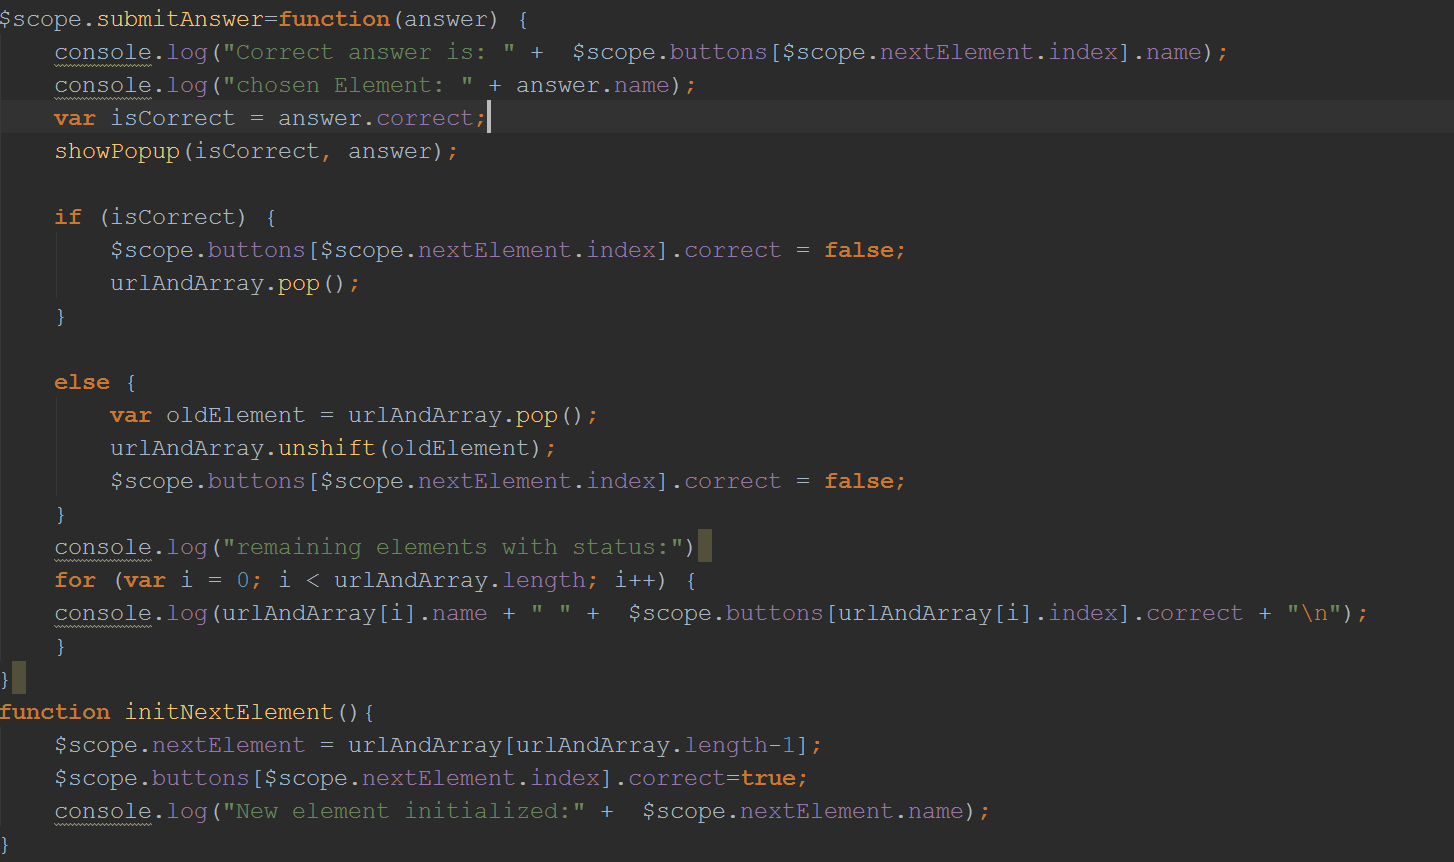
\includegraphics[width=0.5\textwidth]{images/Unit_tests.PNG}
    \caption{Unit test for two functions}
    \label{fig:unit_test}
    
\end{figure}

\begin{figure}[H]
\centering
    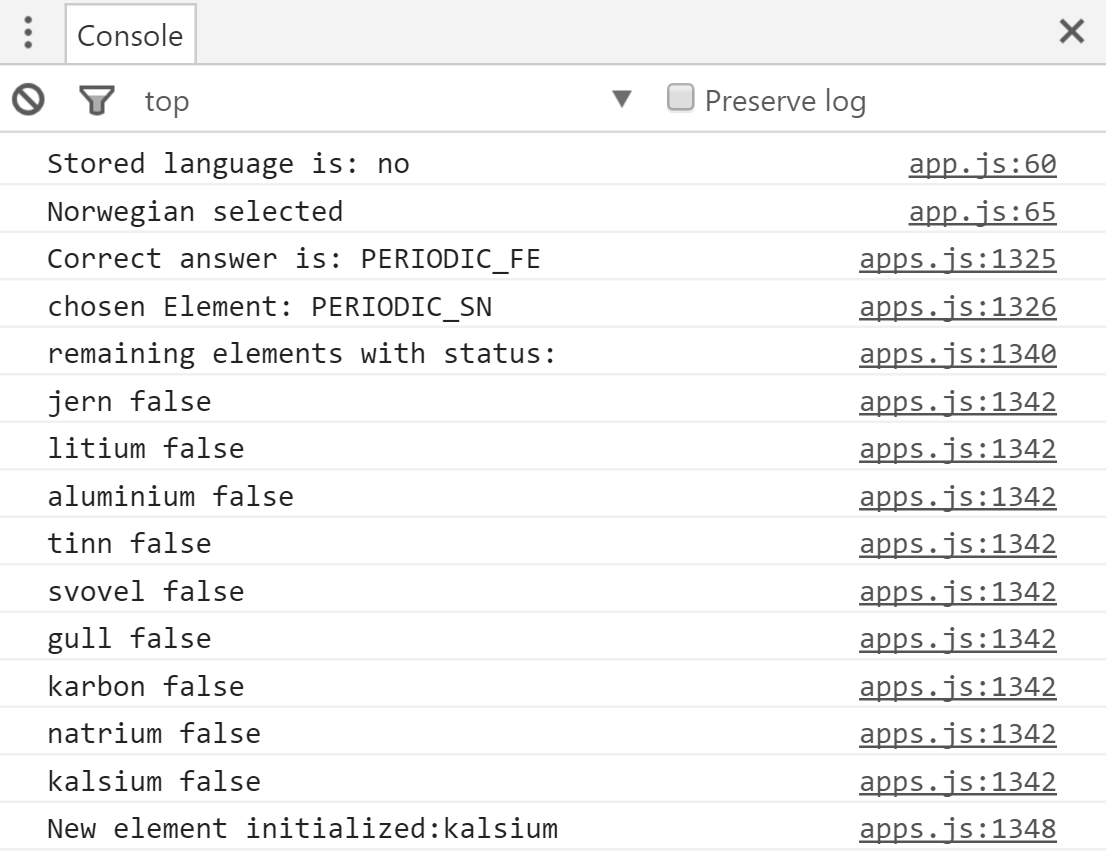
\includegraphics[width=0.5\textwidth]{images/Console_output.PNG}
    \caption{Output from unit tests}
    \label{fig:console_output}
    
\end{figure}

\subsection{Graphical user interface testing}
In this project the GUI testing was done by the group. When a module was completed, it was tested by a member of the group who did not partake in the development of that module. When 5 of the minigames and the overview was finished these were uploaded to a couple of tablets owned by Vitensenteret, so they could perform their own tests and give the group feedback on the next meeting. The team was in contact with an educator employed at the Science Center with insight on necessities when it comes to communicating with children. This was a very useful resource for the group, considering that the main audience are families with children, ages six to ten.\\
\\
Appendix \ref{appendix:TToE} shows the detailed tests that were developed for the ``Elements" minigame. The same kinds of tests were developed and conducted on all modules of the application. But have not been included in this report.

\subsection{User testing}
Initially the group was supposed to perform usability tests towards the end of the project. This would not be in a laboratory, but in the exhibition, under close observation. The plan was to ask families if they were interested in testing our application. The group would follow them and take notes on what they said, how long the different games took to complete and ask them a couple of questions about the experience after they had finished. Time limitations prohibited this from happening. The product was not finished in time to complete the tests, and if they were completed, the group would not be able to change the application after the tests were completed.

\subsection{Integration testing}
The majority of the integration tests were done by the group in preparation for the meetings with the customer. First everyone conduct their own GUI tests for the part of the application they have completed during the iteration. If the GUI tests are passed, integration testing can begin.
\\\\
Integration tests were done in order. One by one, the team members that had something to integrate merged the master branch into their own branch and tested if all of their functionality remained intact, before merging the changes back into the master branch. The reason for doing this and not merging everything to master directly was that this made it easier to figure out where and when an error occurred. The last step in this process was that the last person to integrate conducted a full GUI test in collaboration with the rest of the team.

\subsection{System Testing}
Because the application runs locally on the users phone the application had no system to stress test. The only part of the system the group would consider necessary to stress test was the database the application would send the ``robots" to. This functionality was not implemented, so there was no stress testing.\\
\\
In order to make sure the application could be run on different mobile devices it had to be tested on multiple devices and operating systems. The focus was on smart-phones, rather than tablets, because this was what Vitensenteret considered most important. \\
\\
When running an application on different devices it is very important that it scales correctly with the screen size, resolution, and operating system. In the early phases of development the application was run in a web browser with a simulator, provided by the ionic framework, Ionic Lab. The simulator emulated how the application looked and behaved on both Ios and Android devices(\ref{ref:ioniclab}). This simulator was very useful in the beginning, but because it was limited to a fixed size and resolution, it was not used for long.
\\\\
\begin{figure}[H]\label{ref:ioniclab}
\centering
    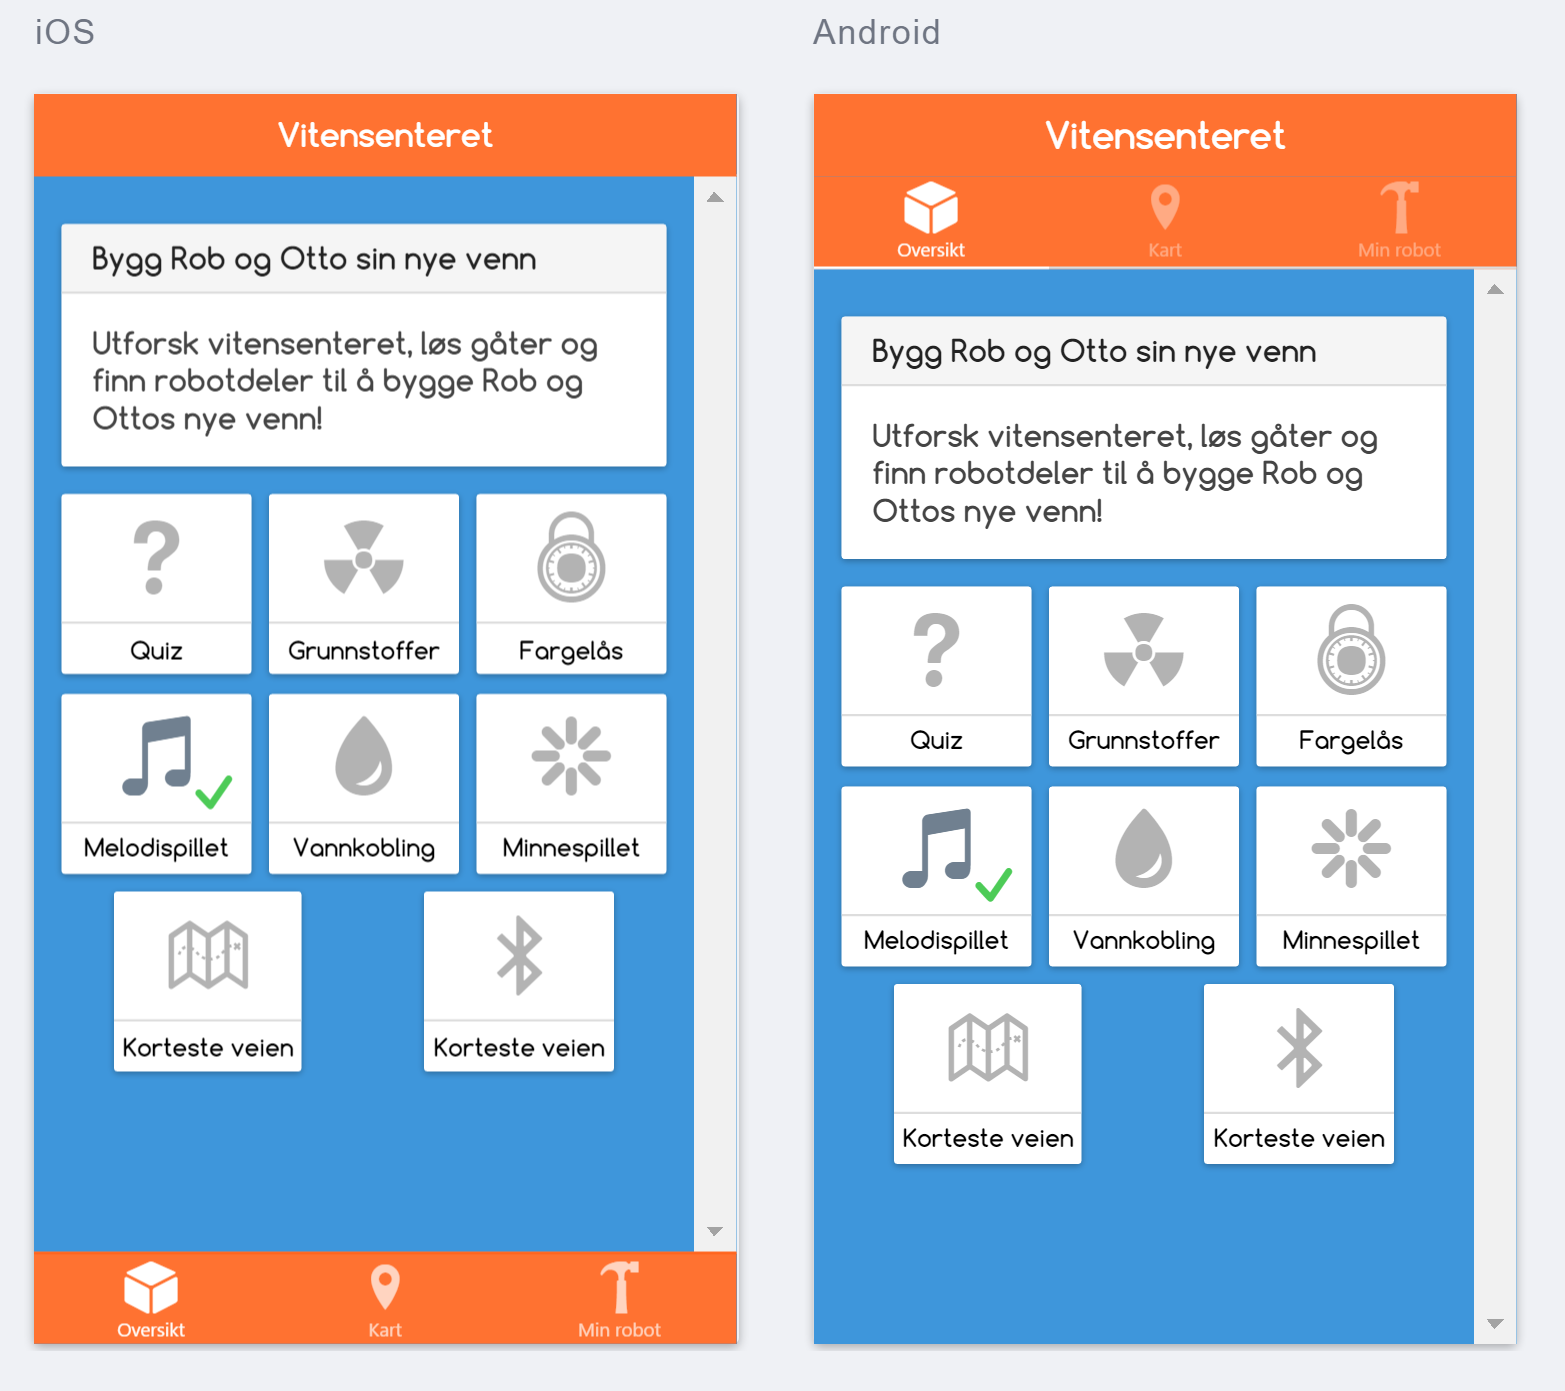
\includegraphics[width=0.5\textwidth]{images/ioniclab.PNG}
    \caption{iOS and Andoid simulation by Ionic Lab}
    \label{fig:console_output}
    
\end{figure}
\\
Ionic Lab was replaced by running the application in ``device mode" in Google Chrome. This provided the group with a simulator that could scale for a set of preset devices, as well as a responsive version, where one could enter the wanted screen resolution. This was used to test for the smallest and larges devices the device could be expected to run on. Figure \ref{fig:chrome_dev} is a screenshot of two chrome browsers in device mode.
\begin{figure}[H]\label{ref:chrome_dev}
\centering
    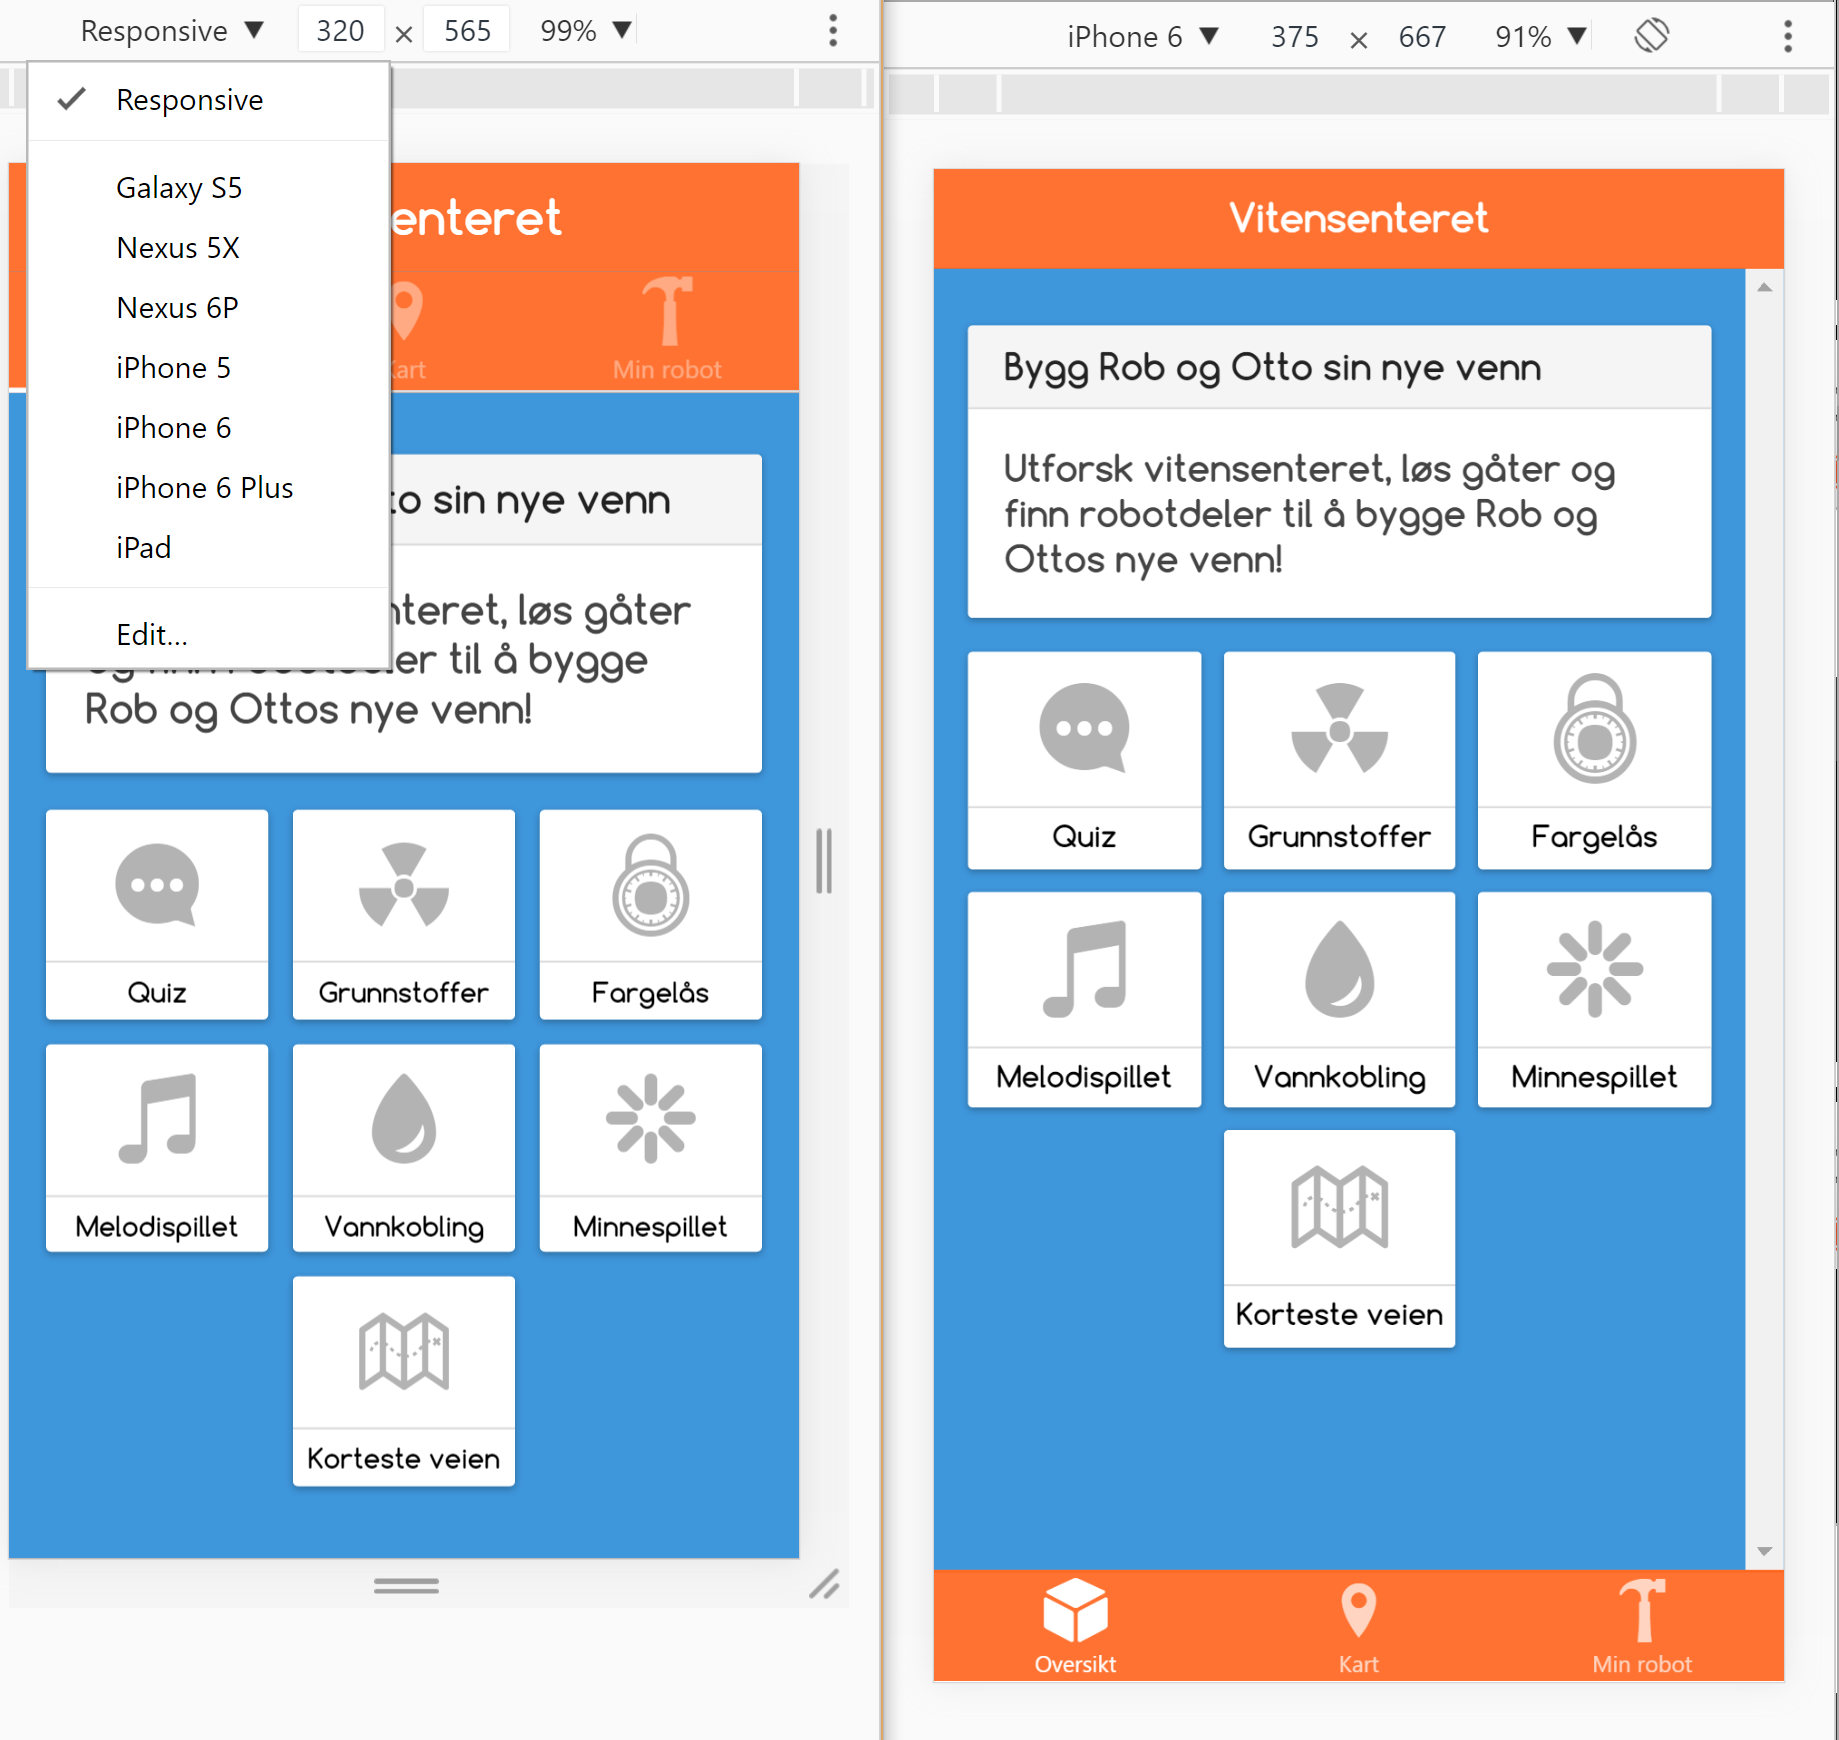
\includegraphics[width=0.5\textwidth]{images/chrome_device.png}
    \caption{Left: simulation showing the different preset resolutions of Google Chromes device mode. Right:Simulation for iPhone6}
    \label{fig:chrome_dev}
\end{figure}
To test how the application performed on devices it was tested on different android smartphones from Samsung and Sony. It was also run on an Iphone 4S. The early tests revealed some scaling issues, that were later fixed. Ideally it would be tested on a broader spectre of devices, but this was what we had available.

\section{Test Results}
\TODO{Her må det skrives noe!!!!!!}

\subsection{Unit testing}
Unit testing was a very useful tool to pinpoint errors and inconsistencies in the code. Every time a unit test failed the group could easily find out what had gone wrong and fix it. By the time the application was finished, all the unit tests were running smoothly. They were later removed because the tests wrote to the console, which the application should not do when it is run.

\subsection{Integration testing}
The group found that our integration method was working well. Considering the amount of changes that were made between the integrations there were not a considerable amount of problems. Occasionally the integration did not go as smooth as the group were hoping, but this was because the merging branch had not been synchronized with the master branch in a long time.

\subsection{System testing}
We did not have the resources to test for all the different versions of Android. But the Android API (level 19) and SDK that was used in the application does not work for Android version lower than KitKat 4.4\cite{AndroidAPI}. In may, 2016, more than 75\% of the worldwide android users were on version 4.4 or higher \cite{AndroidVersions}. Because Norway is a highly technological country and earlier research indicate that Norwegians use the newer android verions \cite{AndroidVersionsNorge} the group speculated that this percentage was higher in Norway, and that it would not be a problem. 

\section{Summary}
The tests the group conducted on our application focused on making sure that all functional and non-functional requirements had been met, rather than focusing on usability and intuitiveness. The reason for this is the lack of time and resources. It was more important for the customer, and the group, that the delivered product was functioning properly than that it was super intuitive and fine tuned. Because of this some types of tests were down prioritized in order for the group to spend time on getting the product to work properly.
\\\\
The application now fulfills all the functional and non-functional requirements, but the group has concluded that there could have been a lot of feedback regarding intuitiveness and design from user testing and user acceptance testing if the group had the time to do them.
